
\documentclass{article}
\usepackage{CTEX}
\usepackage[mathscr]{euscript} 
\usepackage{graphicx}
\usepackage{wrapfig}
\graphicspath{{D:/code/C--practice/image3/}}
\begin{document}
	\section{\kaishu 世界多样性与物质统一性}
		\subsection{\kaishu 物质及其存在方式}
			{\kaishu存在和思维、物质和意识谁为本原的问题何者为第一性的问题}\\
			{\kaishu存在和思维、物质和意识是否具有同一性的问题,即思维能否正确地反应存在、人能否认识或彻底认识世界的问题 }\\
			{\kaishu物质是标志客观实在的哲学范畴,这种客观实在是人通过感觉感知的,它不依赖于我们的感觉而存在,为我们的感觉所复写、摄影、反映 }--{\kaishu物质最本质的规定是客观实在性 坚持了能动的反映论和可知论,批判了不可知论}\\
			{\kaishu 物质的根本属性是运动 运动是标志一切事物和现象的变化及其过程的哲学范畴}\\
			{\kaishu 时间——物质运动的持续性、顺序性}\\
			{\kaishu 空间——物质运动的广延性、伸张性}
		\subsection{\kaishu 物质与意识的辩证关系}
			{\kaishu 意识是人脑的机能和属性,是客观世界的主观映象。物质对意识具有决定作用}\\
			{\kaishu 语言是一种实践的、既为别人存在因而也为我自身而存在的、现实的意识}\\
			{\kaishu 意识是物质的产物,但又不是物质本身}\\
			{\kaishu 意识对物质具有反作用力}\\
			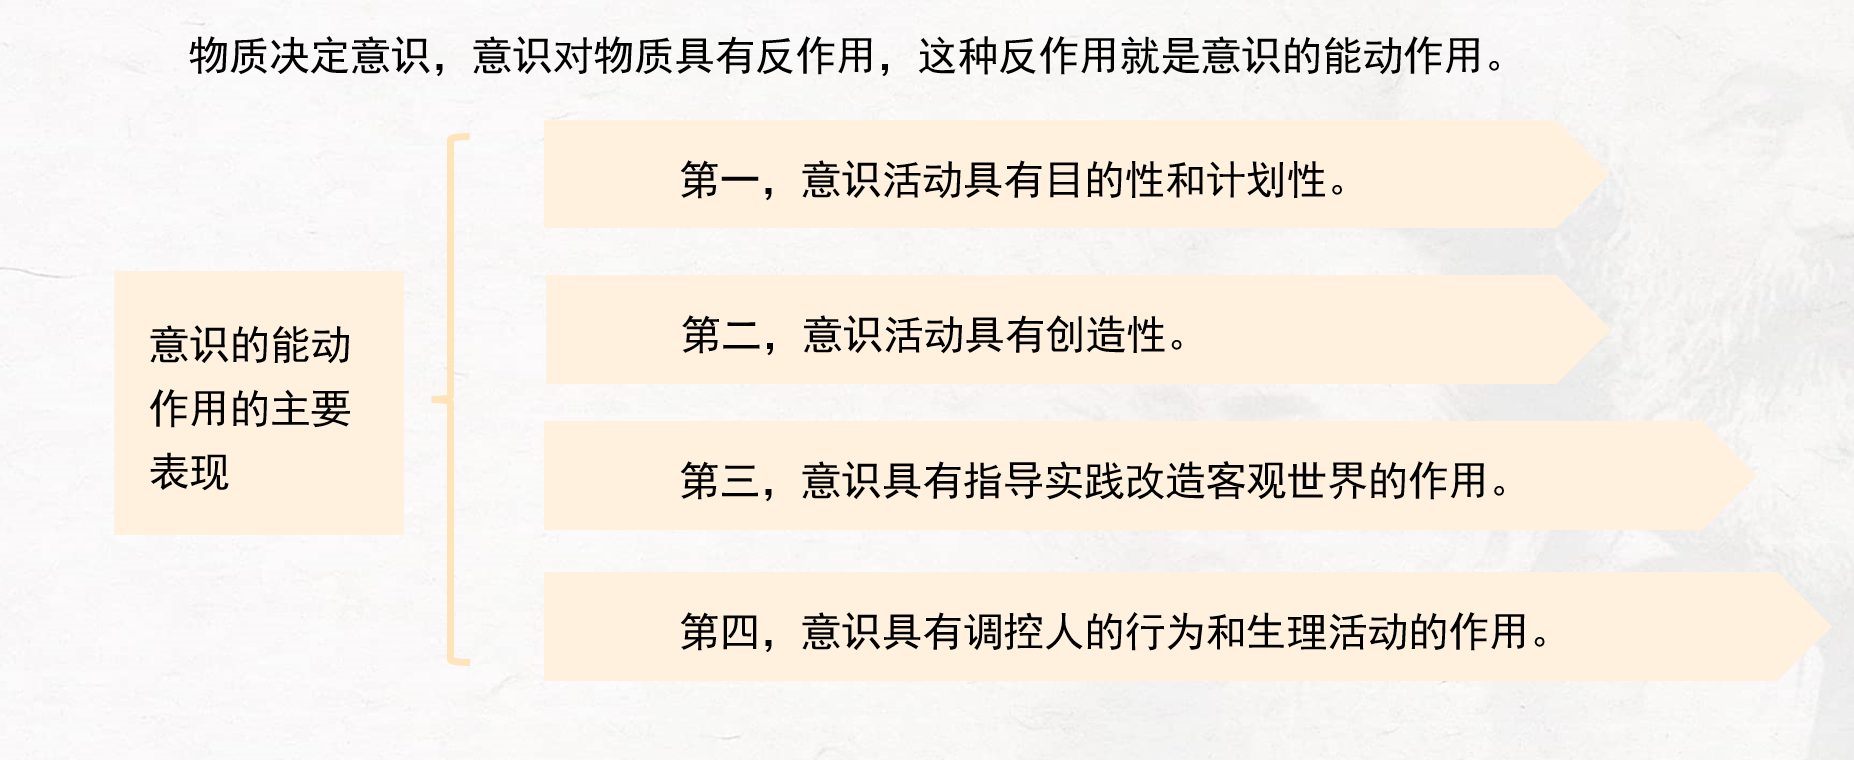
\includegraphics[width=12cm,height=8cm]{reacting force.png}\\
			{\kaishu 主观能动性和客观规律性的辩证统一:1、尊重客观规律是正确发挥主观能动性的前提(规律是事物变化发展过程中本身所固有的内在的、本质的、必然的联系)2、只有充分发挥主观能动性,才能正确认识和利用客观规律-实践是客观规律性与主观能动性统一的基础}\\
		\subsection{\kaishu 世界的物质统一性}
			{\kaishu 物质是世界的本原,世界统一于物质}\\
			{\kaishu 自然界是物质的——人类社会本质上是物质的——人的意识统一于物质}\\
			{\kaishu 我国社会仍处于并将长期处于社会主义初级阶段的基本国情没有变}\\
			{\kaishu 我国社会的主要矛盾发生了变化,已经转化为人民日益增长的美好生活需要和不平衡不充分的发展之间的矛盾}
	\section{\kaishu 事物普遍联系和变化发展}
		\subsection{\kaishu 联系与发展的普遍性}
			{\kaishu唯物辩证法认为,世界上的万事万物都处于普遍联系之中,普遍联系(客观性、普遍性、多样性、条件性(1、条件对事物发展和人的活动具有支持或限制的作用 2、条件是可以改变的 3、改变和创造条件必须尊重事物发展的客观规律))引起了事物的运动发展}\\
			{\kaishu 发展则是事物变化中前进的、上升的运动}\\
			{\kaishu 物质世界的发展,特别是人类社会的发展,其实质是新事物的产生和旧事物的灭亡}
		\subsection{\kaishu 对立统一规律是事物发展的根本规律}
			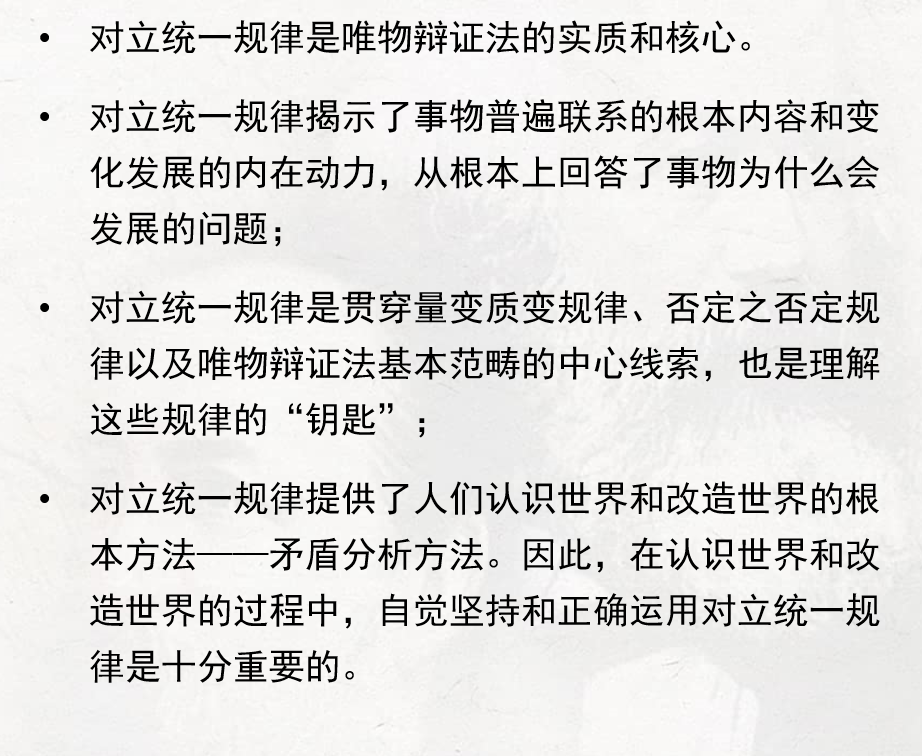
\includegraphics{unity of opposites.png}\\
			{\kaishu 矛盾的对立属性称为斗争性——矛盾的同一属性称为同一性}\\
			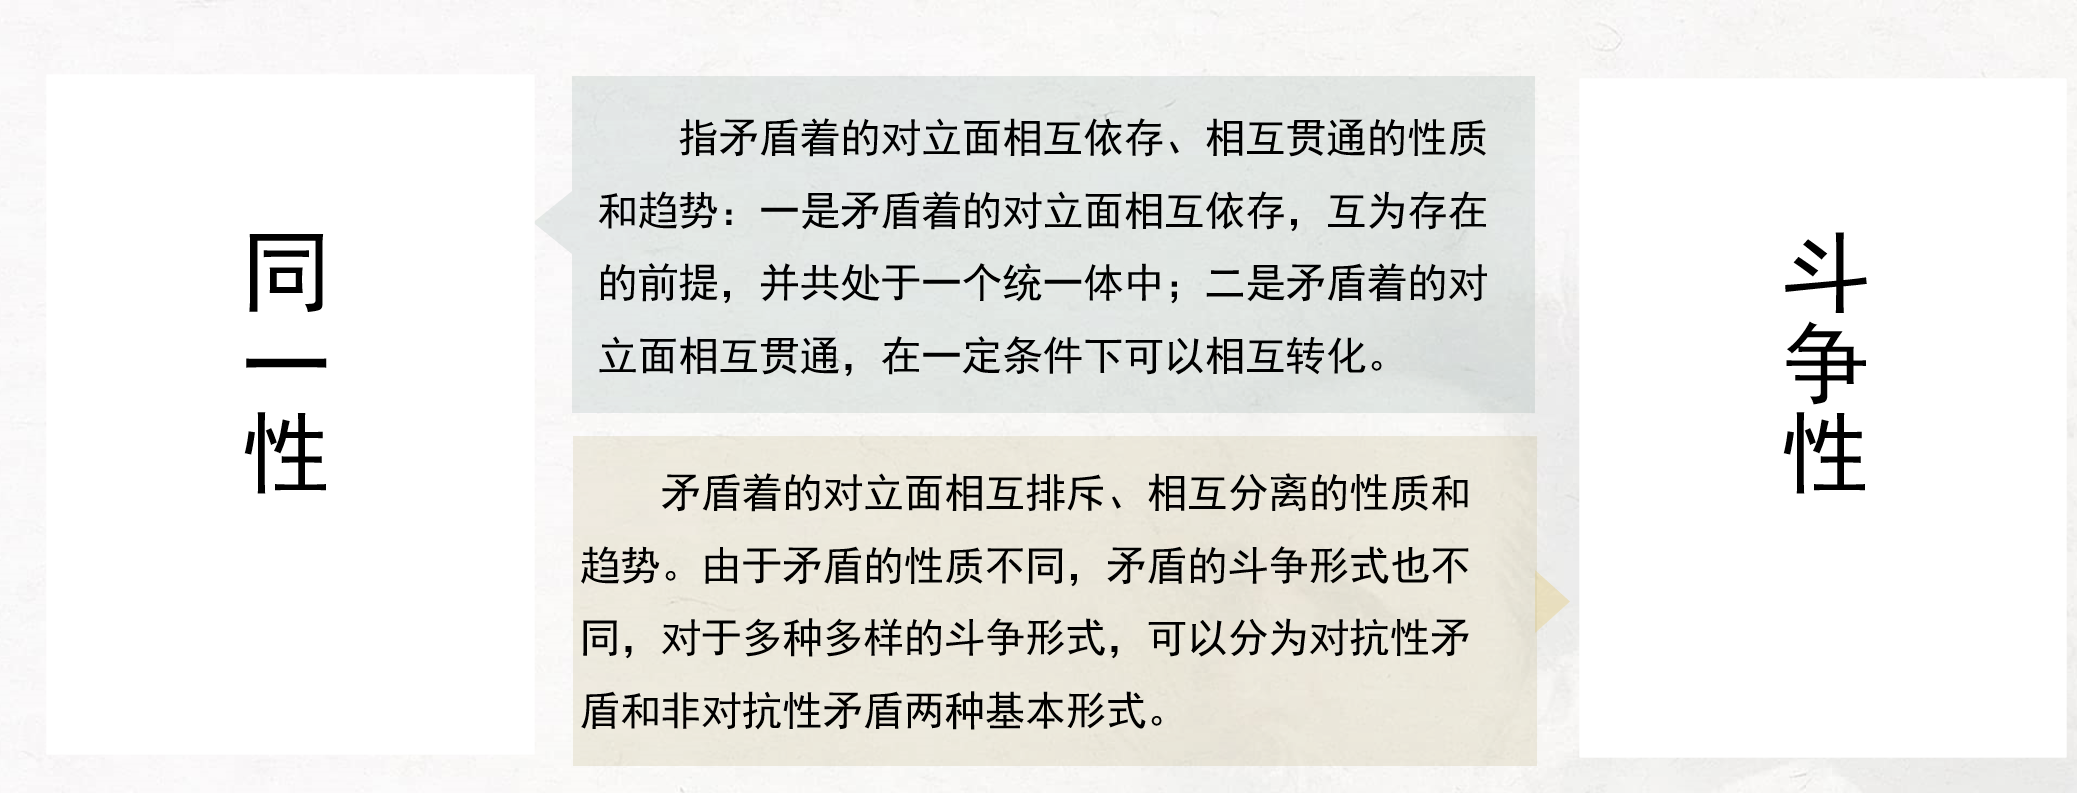
\includegraphics{identity.png}\\
			{\kaishu 矛盾的同一性在事物发展中的作用表现在:第一,同一性是事物存在和发展的前提,在矛盾双方中,一方的发展以另一方的发展为条件,发展是矛盾统一体的发展。第二,同一性使矛盾双方相互吸取有利于自身的因素,在相互作用中各自得到发展。第三,同一性规定着事物转化的可能和发展的趋势。事物之所以能够转化,是由于事物内部矛盾双方具有相互贯通的关系。事物的发展方向、趋势不是随意的,而是有规律地向自己的对立面转化。}
		\subsection{\kaishu量变质变规律和否定之否定规律}
			{\kaishu 量变质变规律 1、量变是事物数量的增减和组成要素排列次序的变动,是保持事物的质的相对稳定性的不显著变化,体现了事物发展渐进过程的连续性。2、质变是事物性质的根本变化,是事物由一种质态向另一种质态的飞跃,体现了事物发展渐进过程和连续性的中断。}\\
			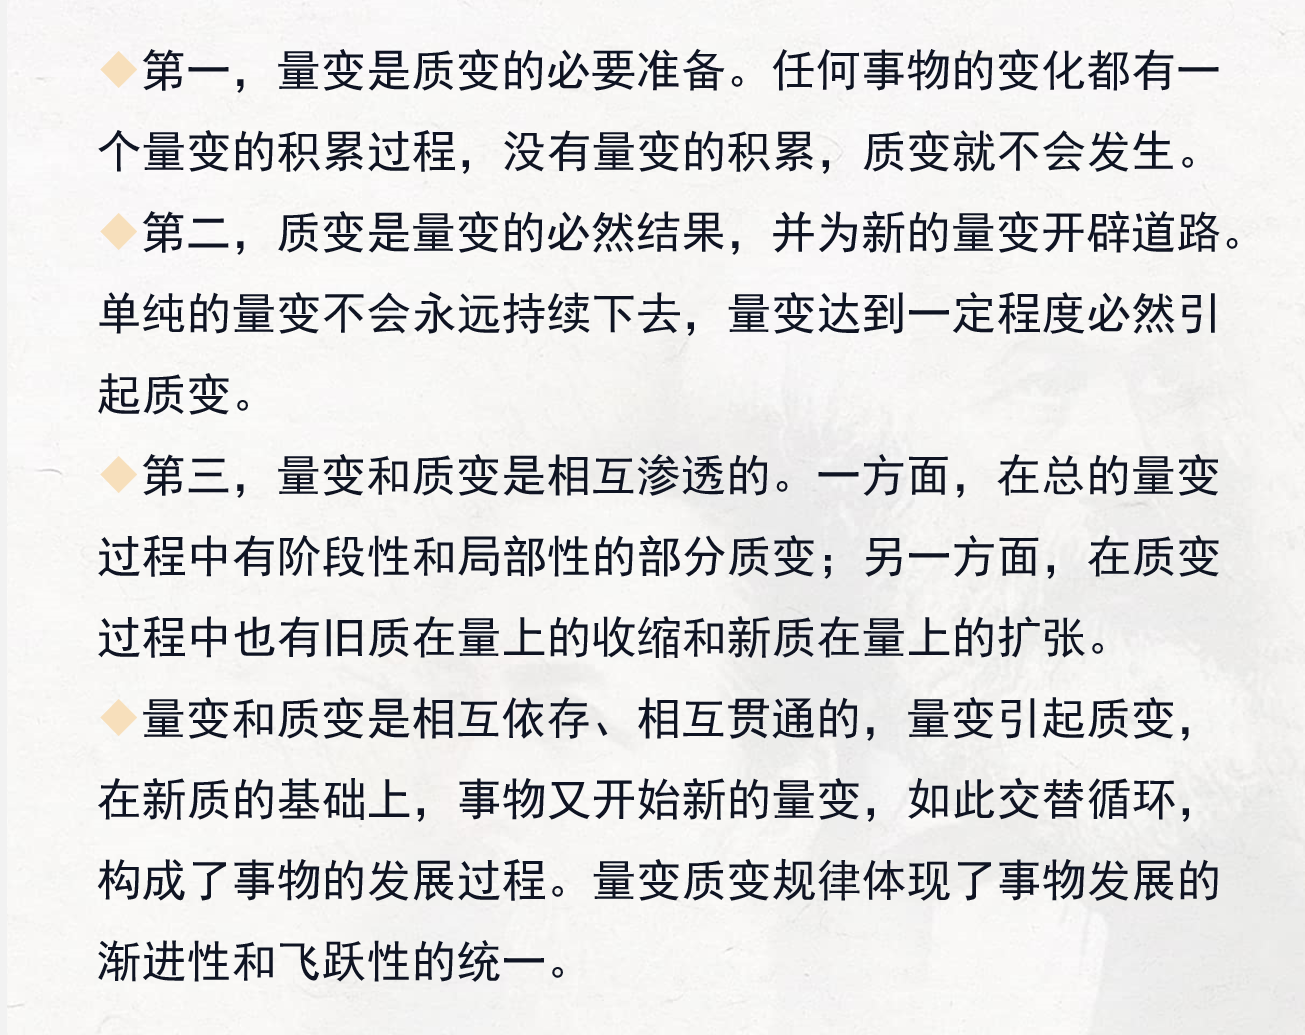
\includegraphics{Quantitative change and qualitative change.png}\\
			{\kaishu 事物的发展是通过其内在矛盾运动以自我否定的方式而实现的}\\
			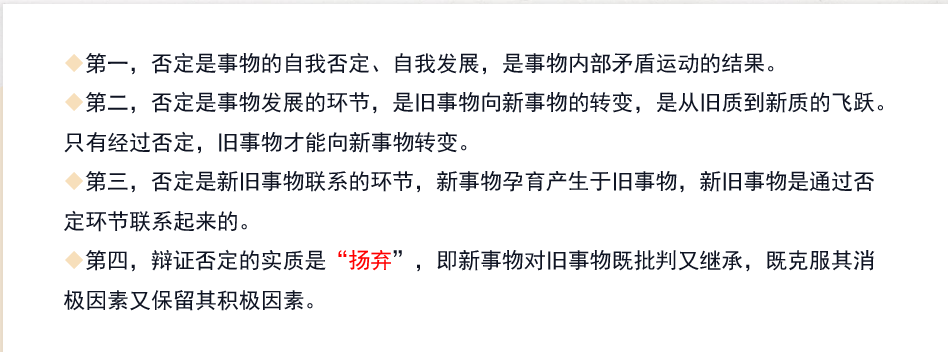
\includegraphics{no.png}\\
			{\kaishu 否定之否定规律揭示了事物发展的前进性与曲折性的统一。前进性体现在每一次否定都是质变,都把事物推进到新阶段;每一个周期都是开放的,前一个周期的终点是下一个周期的起点,不存在不被否定的终点。曲折性体现在回复性上,其中有暂时的停顿甚至是倒退。这表明,事物的发展不是直线式前进,而是螺旋式上升的。}\\
		\subsection{\kaishu联系和发展的基本环节}
			{\kaishu 内容和形式是从构成要素和表现方式上反映事物的一对基本范畴}\\
			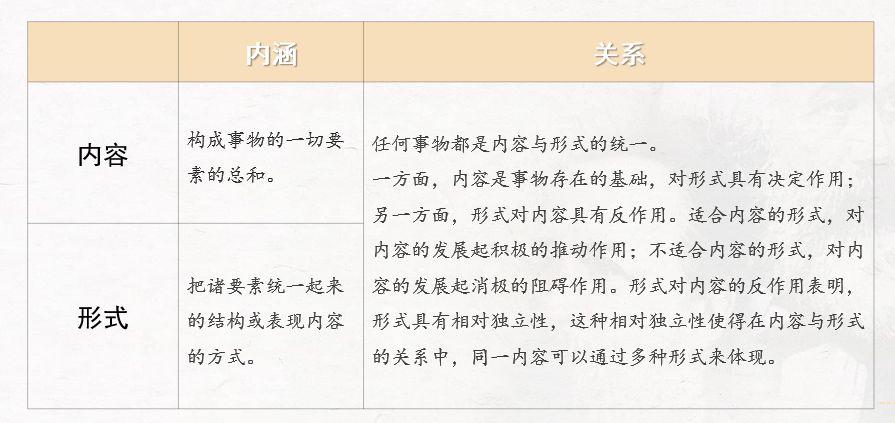
\includegraphics{content form.png}\\
			{\kaishu 内容与形式的矛盾贯穿于事物发展过程的始终,从最初的基本适合到基本不适合,随着矛盾的解决,再到新的基本适合。在我们的认识和实践中,要根据内容决定形式的原理,注重事物的内容,反对忽视内容、夸大形式作用的形式主义;又要积极利用合适的形式去促进内容的发展,不能忽视形式对内容的能动促进作用。}\\
			{\kaishu 本质与现象是揭示事物内在联系和外在表现的一对范畴}\\
			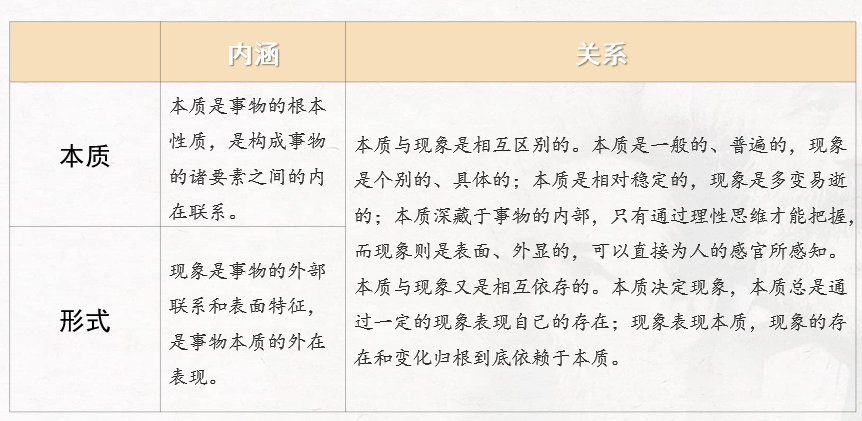
\includegraphics{essence form.png}\\
			{\kaishu 原因与结果是揭示事物引起和被引起关系的一对范畴}\\
			{\kaishu 必然和偶然是揭示事物产生、发展和衰亡过程中的不同趋势的一对范畴}\\
			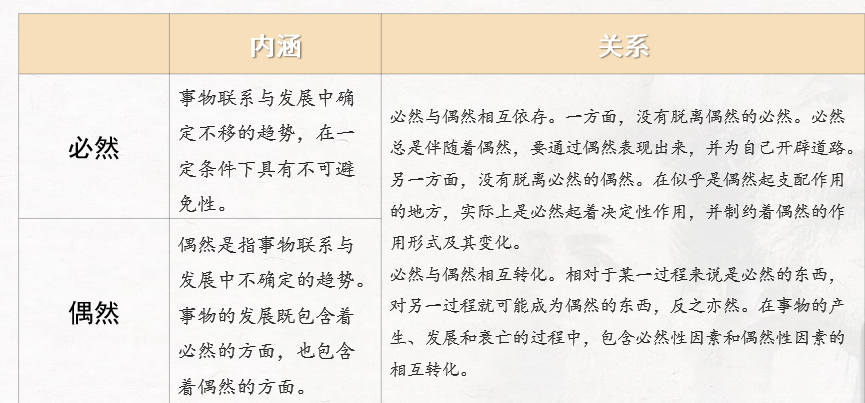
\includegraphics{necessity and contingency.png}\\
			{\kaishu 现实与可能是反映事物的过去、现在和将来关系的一对范畴}\\
			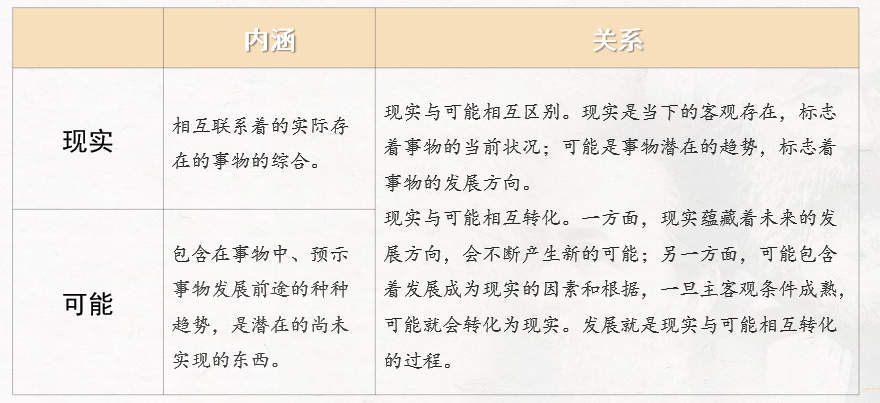
\includegraphics{reality and potential.png}\\
	\section{\kaishu 唯物辩证法是认识世界和改造世界的根本方法}
		\subsection{唯物辩证法的本质特征和认识功能}
			{\kaishu 唯物辩证法本质上是批判的和革命的}\\
			{\kaishu 辩证法在对现存事物的肯定的理解中同时包含对现存事物的否定的理解,即对现存事物的必然灭亡的理解——在它面前,除了生成和灭亡的不断过程、无止境地由低级上升到高级的不断过程,什么都不存在}\\
			{\kaishu 唯物论和辩证法的统一体现为客观辩证法与主观辩证法的统一}\\
			\includegraphics{subjective and objective.png}\\
			{\kaishu 所谓的客观辩证法是在整个自然界中起支配作用的,而所谓的主观辩证法,即辩证的思维,不过是在自然界中到处发生作用的、对立中的运动的反映。——恩格斯}\\
			{\kaishu 唯物辩证法是科学的认识方法}\\
			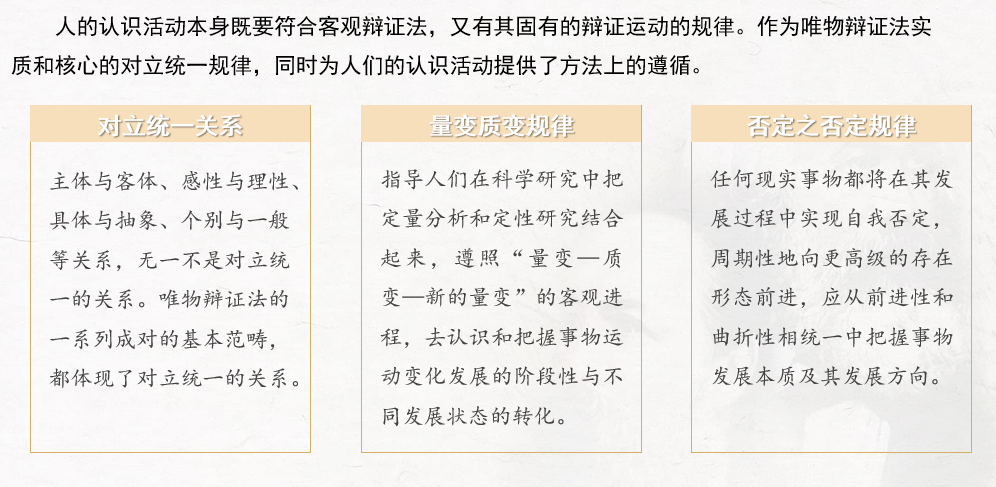
\includegraphics{summary.png}\\
			{\kaishu 唯物辩证法是科学的认识方法}
		\subsection{辩证思维方法与现代科学思维方法}
			{\kaishu 辩证思维方法是现代科学思维方法的基础和原则,现代科学思维方法是辩证思维方法的深化和展开,要善于把二者结合起来完整地把握}\\
			{\kaishu 归纳与演绎是人类思维从个别到一般,又由一般到个别的最常见的推理形式}\\
			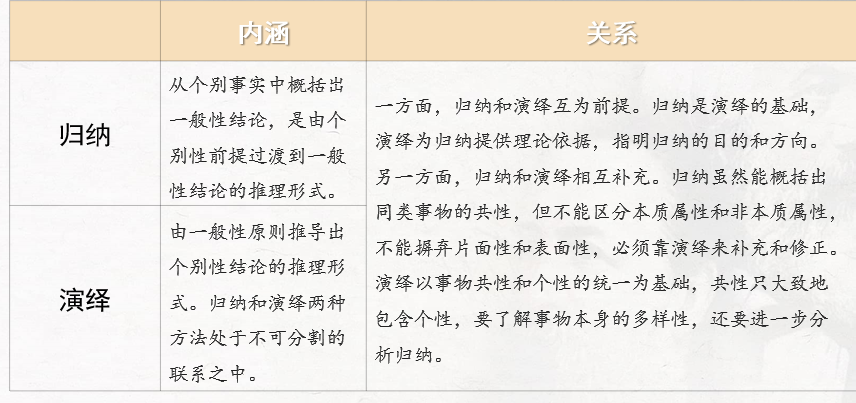
\includegraphics{induction and deduction.png}\\
			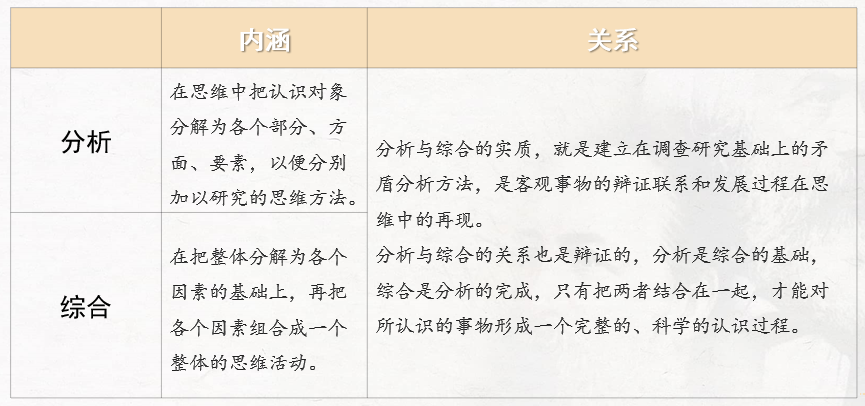
\includegraphics{analyse and comprehensive.png}\\
			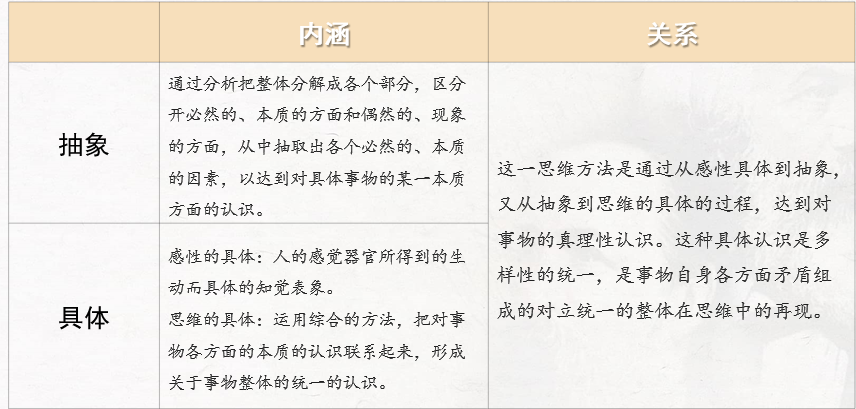
\includegraphics{abstract and concrete.png}\\
			\includegraphics{history and logic.png}\\
			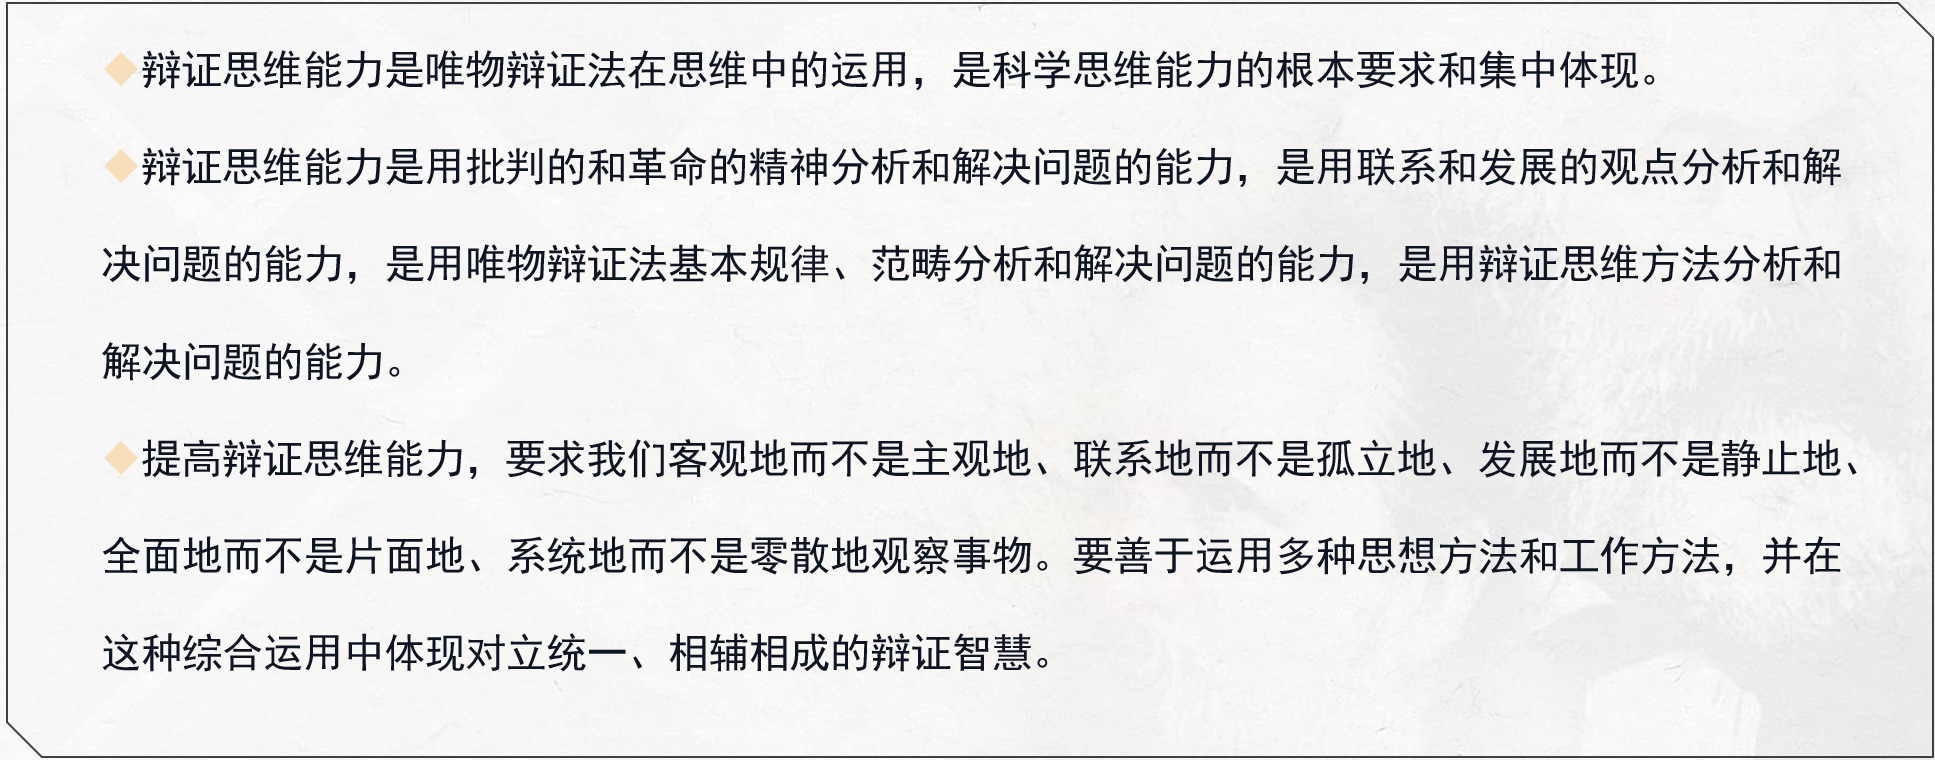
\includegraphics{dialectial thinking.png}\\
			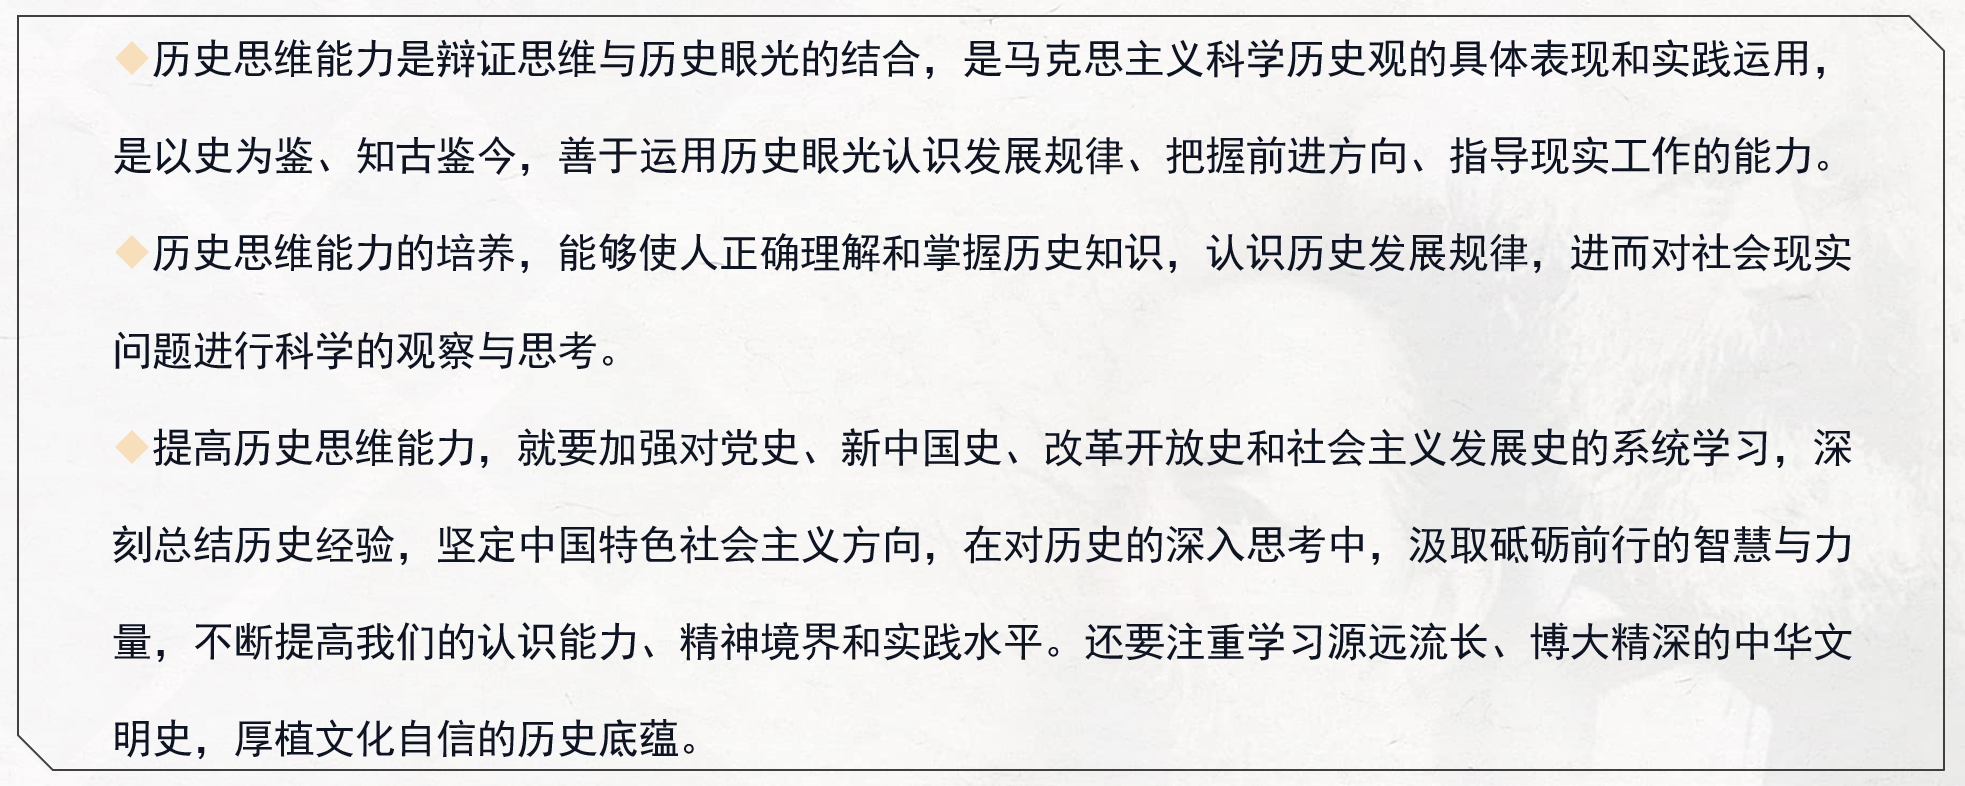
\includegraphics{historical thinking.png}\\
			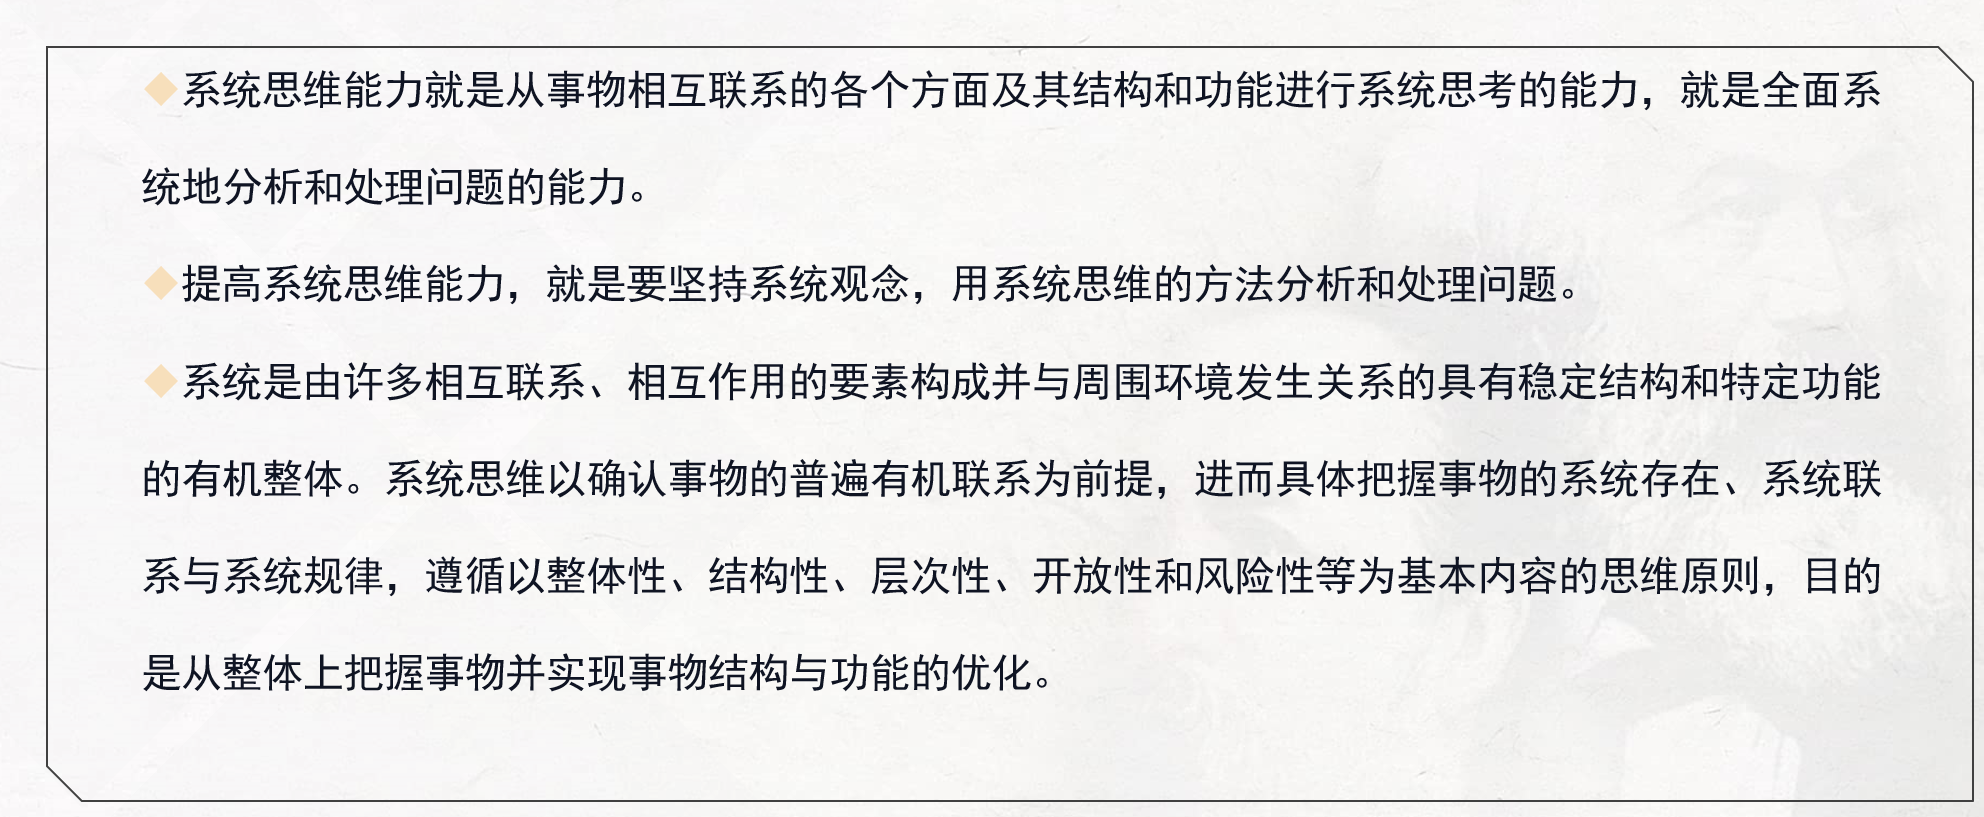
\includegraphics{systematic thinking.png}\\
			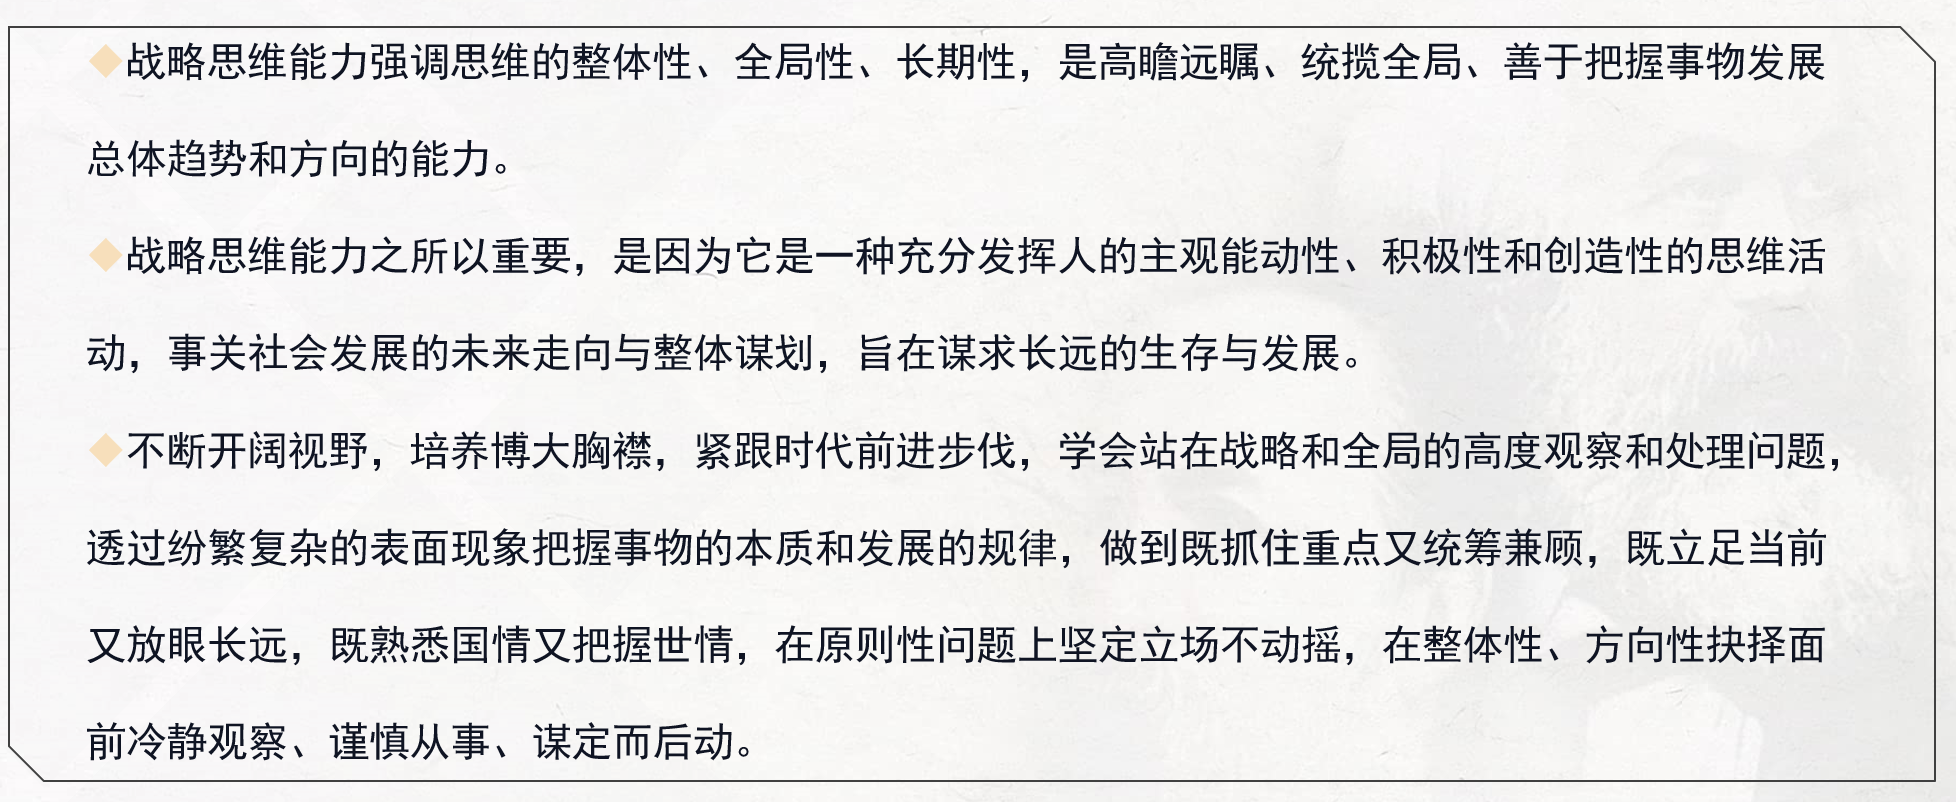
\includegraphics{strategic thinking.png}\\
			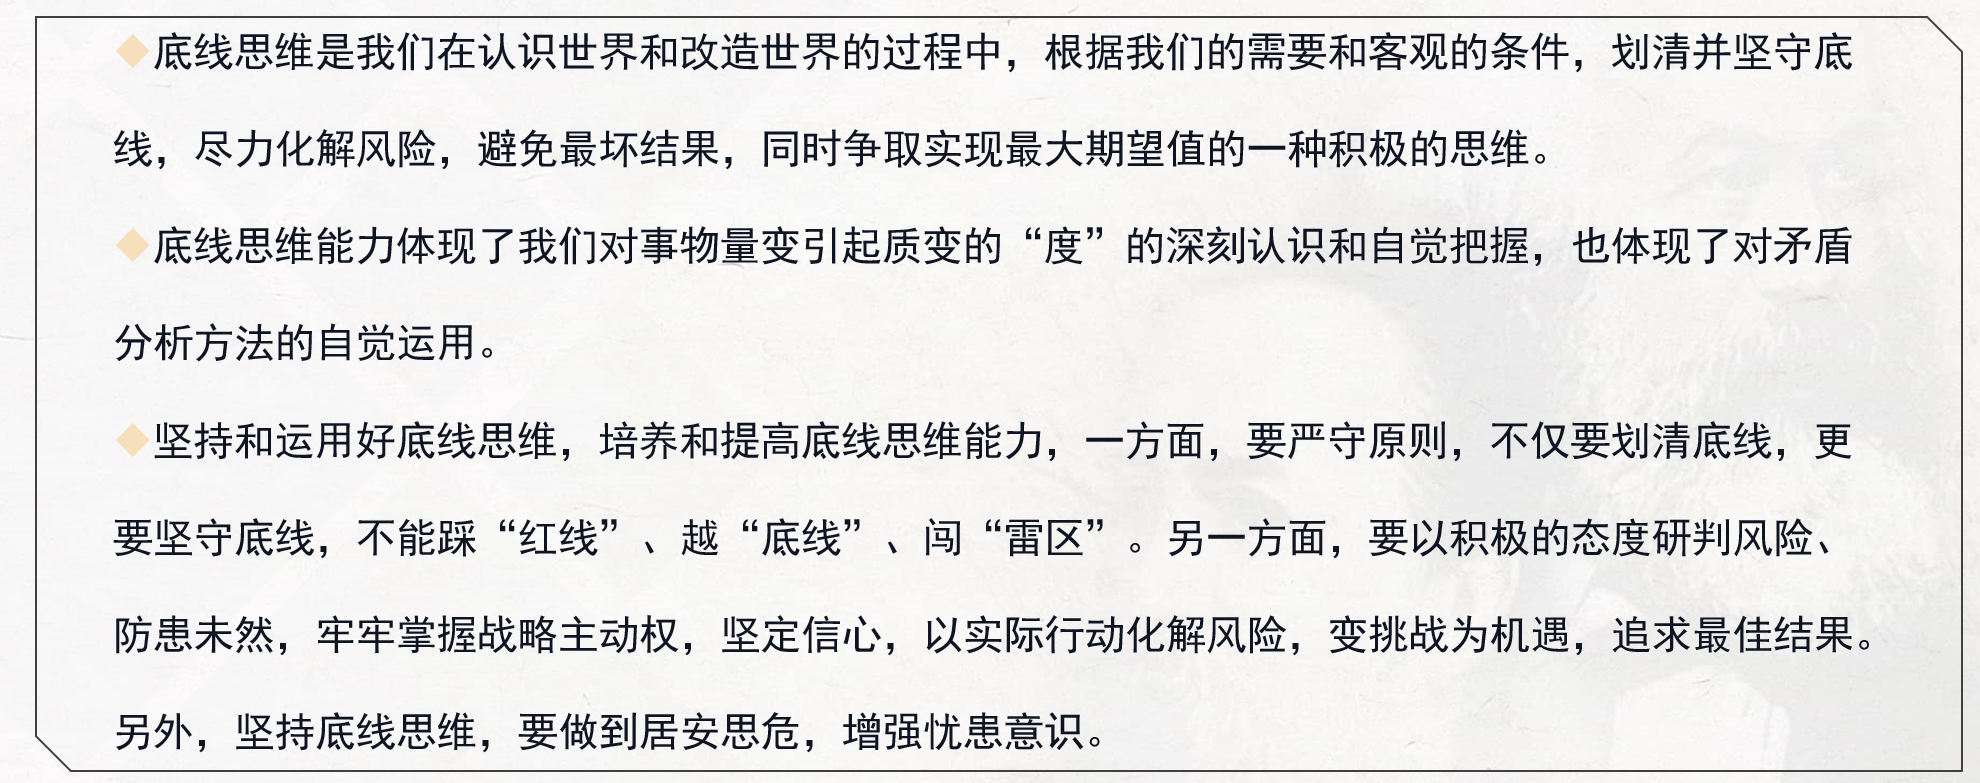
\includegraphics{Bottom-line thinking.png}\\
			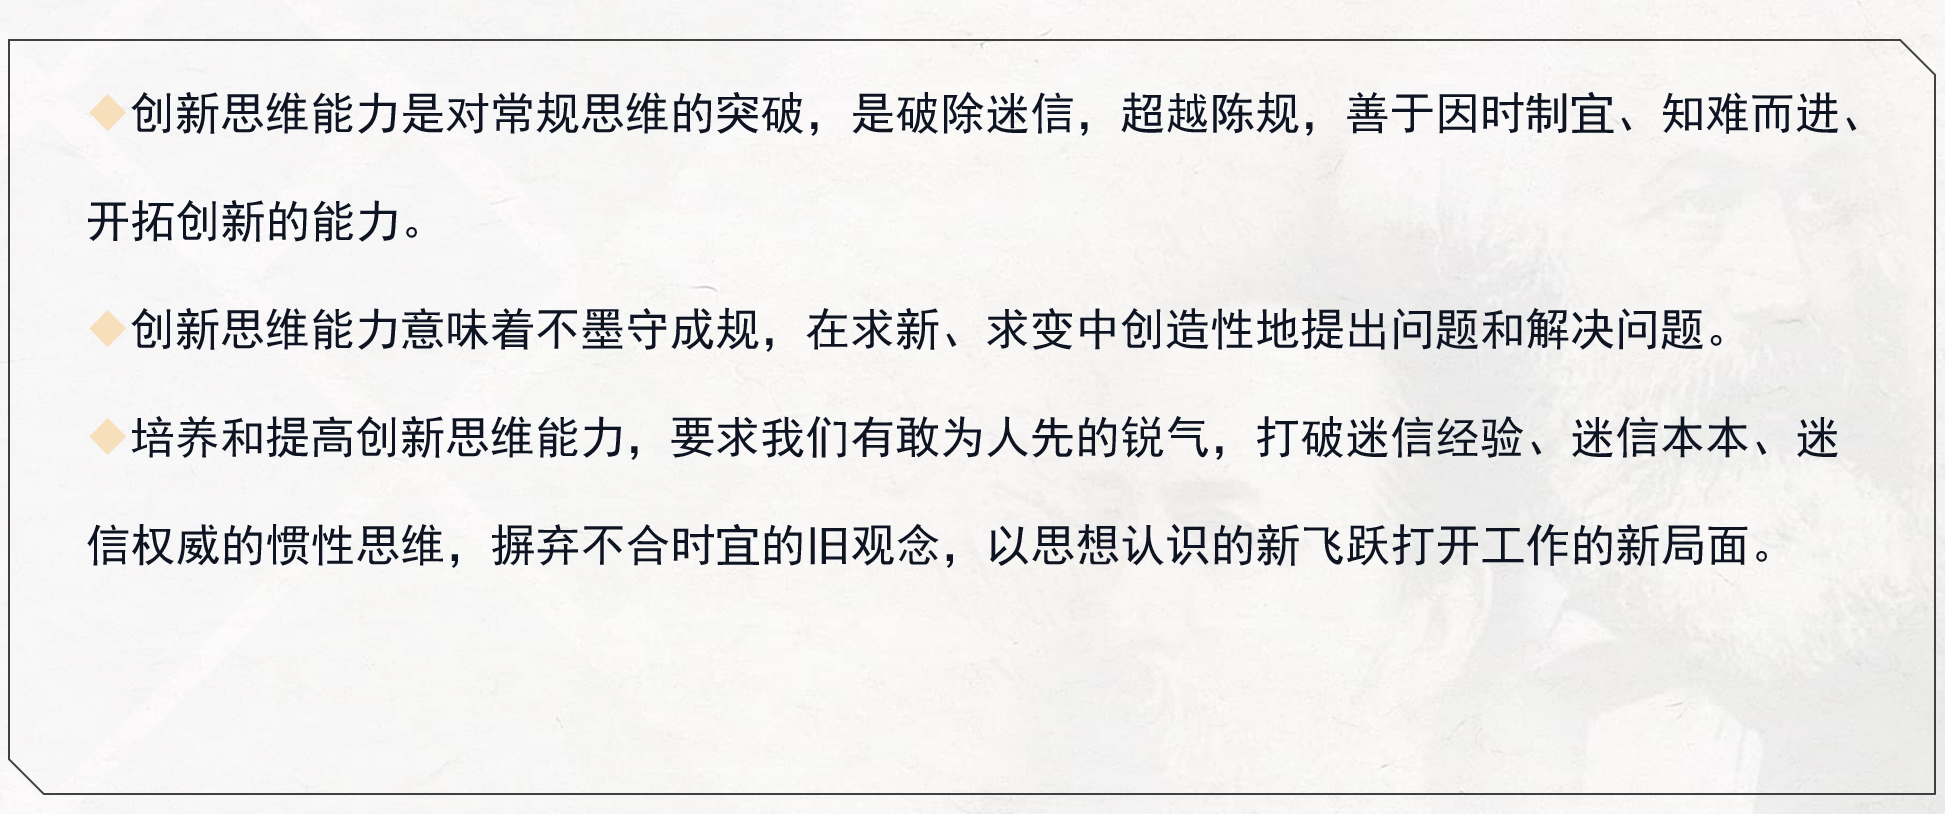
\includegraphics{innovative thinking.png}
\end{document}

